% !TEX program = xelatex
\documentclass[12pt]{article}


% Language setting
% Replace `english' with e.g. `spanish' to change the document language
\usepackage[english]{babel}
\usepackage{xeCJK}
\usepackage{CJKutf8}
\usepackage{svg}

% Set page size and margins
% Replace `letterpaper' with `a4paper' for UK/EU standard size
\usepackage[a4paper,top=2cm,bottom=2cm,left=3cm,right=3cm ,marginparwidth=1.75cm]{geometry}

% Useful packages
\usepackage{amsmath}
\usepackage{graphicx}
\usepackage[colorlinks=true, allcolors=blue]{hyperref}

\usepackage{array}
\newcolumntype{P}[1]{>{\centering\arraybackslash}p{#1}}
\newcolumntype{M}[1]{>{\centering\arraybackslash}m{#1}}


% \usepackage{subfigure}
\usepackage{adjustbox}

\usepackage{caption}
\usepackage{subcaption}

\usepackage{siunitx}

\usepackage{float}
\usepackage{subfloat}

% ----- paragraph -----
\usepackage{titlesec}
\setcounter{secnumdepth}{4}
\titleformat{\paragraph}
{\normalfont\normalsize\bfseries}{\theparagraph}{1em}{}
\titlespacing*{\paragraph}
{0pt}{3.25ex plus 1ex minus .2ex}{1.5ex plus .2ex}
% ----- paragraph ----

% \setCJKmainfont{NotoSansCJKtc-DemiLight.otf}
% \setCJKmainfont{NotoSerifTC-Black.otf}
% \setCJKmainfont{NotoSerifTC-Regular.otf}
% \setCJKmainfont{NotoSerifTC-Bold.otf}
\setCJKmainfont{NotoSerifTC-Regular}

\usepackage{indentfirst}
\setlength\parindent{24pt}


\begin{document}

% \maketitle

\begin{titlepage}
   \begin{center}
       \vspace*{1cm}
        \begin{LARGE}  
            \textbf{
            \\ 數位電路實驗結報一
            \\ \
            \\ --6-bit 數位加法器--
            }
        \end{LARGE}
       \vspace{0.5cm}
         \textbf{}
            
       \vspace{1.5cm}

       % \begin{CJK}{UTF-8}{bsmi}
       \textbf{Group 2: B11303052 蘇盈翰 (Right), B11702091 張容爾 (Middle), B10901144 王俊皓(Left)}
        % \end{CJK}
         
       \vspace{1.5cm}

       \text{\today}

       \vspace{0.8cm}

       
\includegraphics[width=0.7\textwidth]{figure/Member.jpg}
       
       \vfill
            
       \vspace{0.8cm}
       
   \end{center}
\end{titlepage}

\section{實驗理論與原理}

\subsection{半加器與全加器 (Half Adder \& Full Adder)}
加法器為數位邏輯電路中執行二進位加法運算之核心組件。最基本的\textbf{半加器}負責兩個單一位元 $A$ 與 $B$ 的加法，其輸出包含總和 ($S$) 與進位 ($C_{out}$)，布林邏輯表示式為：
\begin{align}
    \mathrm{S} &= \mathrm{A} \oplus \mathrm{B} \\
    \mathrm{C_{out}} &= \mathrm{A} \cdot \mathrm{B}
\end{align}

為了處理多位元的加法，必須考慮來自較低位元的進位。因此引入了\textbf{全加器}，它包含三個輸入端：兩個加數 ($A, B$) 以及一個進位輸入 ($C_{in}$)。全加器的輸出邏輯表示式為：
\begin{align}
    \mathrm{S} &= \mathrm{A} \oplus \mathrm{B} \oplus \mathrm{C_{in}} \\
    \mathrm{C_{out}} &= (\mathrm{A} \cdot \mathrm{B}) + (\mathrm{C_{in}} \cdot (\mathrm{A} \oplus \mathrm{B}))
\end{align}

\subsection{邏輯閘實現與笛摩根定理}
在實體電路佈線中，我們使用 IC 7486 (XOR 閘) 與 IC 7400 (NAND 閘) 來建構上述邏輯。總和 $S$ 可直接透過兩個 XOR 閘串接完成。

對於進位 $C_{out}$ 的部分，原本的設計需要 AND 閘與 OR 閘。為了僅使用 NAND 閘 (IC 7400) 來完成進位電路，我們可套用\textbf{笛摩根定理 (De Morgan's Laws)} 將原本的 AND-OR 形式轉換為 NAND-NAND 形式：
\begin{equation}
    C_{out} = \overline{ \overline{(A \cdot B)} \cdot \overline{(C_{in} \cdot (A \oplus B))} }
\end{equation}
透過此轉換，即可大幅簡化所需的 IC 種類，完全依靠 7486 與 7400 實現 1-bit 全加器。

\subsection{漣波進位加法器 (Ripple Carry Adder)}
要實現多位元（如本實驗之 6-bit）的加法運算，可將多個全加器串聯組成「漣波進位加法器」。其核心原理是將第 $i$ 個位元的進位輸出 ($C_{out, i}$) 直接連接至第 $i+1$ 個位元的進位輸入 ($C_{in, i+1}$)。

本次實驗中，我們將兩個現成的 3-bit 加法器模組進行擴充，把低位元 (Lower 3-bits) 加法器的最高位進位輸出，連接至高位元 (Upper 3-bits) 加法器的最低位進位輸入 ($C_{in}$)，藉由進位訊號的傳遞 (Carry Propagation)，成功構建出完整的 6-bit 數位加法器。

\section{實驗架設與步驟}

\subsection{1-bit 數位加法器實作 (實驗一)}
\begin{enumerate}
    \item \textbf{硬體接線：}
    \begin{itemize}
        \item 準備 IC 7486 (XOR) 與 IC 7400 (NAND)，將其固定於麵包板上。分別將兩顆 IC 的第 14 腳位連接至 ADALM2000 提供的 +5V 電源 (VCC)，第 7 腳位連接至接地 (GND)。
        \item 依據理論化簡後之電路圖進行佈線：利用 7486 負責處理總和 ($S$) 與部分進位邏輯，並將其輸出結果接入 7400 進行 NAND 邏輯運算，以產生最終的進位輸出 ($C_{out}$)。
        \item 將 ADALM2000 的數位腳位 (DIO) 連接至電路對應節點：DIO 0 接至輸入 $A$、DIO 1 接至輸入 $B$、DIO 2 接至輸入 $C_{in}$；量測端的部分，將 DIO 3 接至總和輸出 $S$、DIO 4 接至進位輸出 $C_{out}$。
    \end{itemize}
    \begin{center}
        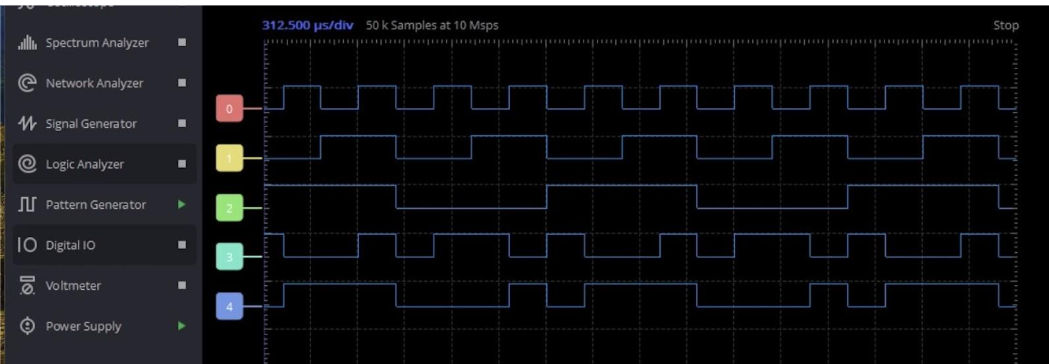
\includegraphics[width=0.7\textwidth]{figure/output wave front.png}
    \end{center}
    \begin{center}
        \begin{table}[H]
    \centering
    \renewcommand{\arraystretch}{1.2} % 增加行高，讓表格看起來不那麼擁擠
    \begin{tabular}{|c||c|c|c|c|c|c|c|c|}
        \hline
        \textbf{狀態} & \textbf{1st} & \textbf{2nd} & \textbf{3rd} & \textbf{4th} & \textbf{5th} & \textbf{6th} & \textbf{7th} & \textbf{8th} \\ \hline \hline
        \textbf{A}    & 1 & 0 & 1 & 0 & 1 & 0 & 1 & 0 \\ \hline
        \textbf{B}    & 0 & 1 & 1 & 0 & 0 & 1 & 1 & 0 \\ \hline
        \textbf{Cin}  & 1 & 1 & 1 & 0 & 0 & 0 & 0 & 1 \\ \hline
        \textbf{S}    & 0 & 0 & 1 & 0 & 1 & 1 & 0 & 1 \\ \hline
        \textbf{Cout} & 1 & 1 & 1 & 0 & 0 & 0 & 1 & 0 \\ \hline
        \end{tabular}
        \caption{1-bit 全加器輸入與輸出之實測真值表}
        \label{tab:truth_table}
    \end{table}
    \end{center}
    
    \item \textbf{軟體設定 (Scopy)：}
    \begin{itemize}
        \item \textbf{Pattern Generator (訊號產生器)：} 開啟 Scopy 軟體，將 DIO 0、1、2 設定為 Binary Counter 模式，並設定為三個等比頻率（例如 $A$ 設為 4 kHz、$B$ 設為 2 kHz、$C_{in}$ 設為 1 kHz）。此設定可產生所有 8 種 0 與 1 的輸入排列組合。
        \item \textbf{Logic Analyzer (邏輯分析儀)：} 開啟 DIO 0 至 DIO 4 的波形顯示。將取樣率 (Sample Rate) 設定為 5 Msps，取樣數量 (Nr of samples) 設定為 20k Samples。
        \item 擷取波形，觀察輸出腳位與輸入腳位之電位變化，並比對全加器真值表以驗證硬體邏輯。
    \end{itemize}
\end{enumerate}

\subsection{多位元加法器串聯測試 (實驗二與延伸)}
\begin{enumerate}
    \item \textbf{3-bit 加法器模組測試：} 取得助教事先製作的 3-bit 加法器電路板，透過板上的指撥開關給定不同的輸入組合，並觀察 LED 燈亮的狀態來驗證 3-bit 的加法結果（例如測試 $3+5=8$，即二進位之 $011_2 + 101_2 = 1000_2$）。
    \item \textbf{6-bit 加法器擴充：} 將兩塊 3-bit 加法器模組進行串聯。把處理低位元 (Lower 3-bits) 模組的進位輸出端 ($C_{out}$)，利用跳線連接至處理高位元 (Upper 3-bits) 模組的進位輸入端 ($C_{in}$)。
    \item 透過 ADALM 再次進行輸入測試，確認進位訊號能順利跨模組傳遞，完成並驗證完整的 6-bit 加法運算邏輯。
\end{enumerate}

\section{實驗結果與分析}


\section{問提與討論}

\subsection{如何使用二進位表示負數?}
\subsection{如何用數位電路實現乘法、 指數運算?}
\subsection{進行多位元加法時 (如實驗二)，可能會遇到哪些問題或限制？商
用電路有什麼優化電路的方式嗎？
}


\section{總結} 


\end{document} 
